\documentclass{beamer}
\usepackage[utf8]{inputenc}
\usepackage[spanish]{babel}
\usepackage{graphicx}
\usepackage{booktabs}
\usepackage{multicol}
\usepackage{amsmath}
\usepackage{hyperref}
\usepackage{changes}

\usetheme{Madrid}

\title{Estabilidad de Redes Financieras Bajo Incertidumbre Tecnológica}
\author{Hernán Venegas \\ Profesor Guía: Sebastián Cea}
\date{27 de junio de 2025 \\ Universidad de Los Andes}

\begin{document}

\frame{\titlepage}

\begin{frame}{Antecedentes: Blockchain vs Sistemas Tradicionales}
\begin{itemize}
    \item \textbf{Sistemas Tradicionales:}
    \begin{itemize}
        \item Ofrecen \textcolor{blue}{estabilidad y confianza} institucional respaldada por marcos regulatorios.
        \item Altos costos debido a la intermediación (bancos, brokers).
    \end{itemize}
    
    \item \textbf{Revolución Tecnológica:}
    \begin{itemize}
        \item Emerge Blockchain en 1991, Bitcoin en 2008 y el concepto de finanzas descentralizadas (DeFi) en 2017.
    \end{itemize}
    
    
    
    \item \textbf{Blockchain:}
    \begin{itemize}
        \item Ofrece \textcolor{blue}{transacciones directas, sin intermediarios}, con mayor transparencia y trazabilidad. Y \textcolor{blue}{menores costos}.
        \item Pero, presenta riesgos de seguridad, volatilidad y potencial lentitud.
    \end{itemize}
\end{itemize}
\end{frame}

    \begin{frame}{Antecedentes: Blockchain vs Sistemas Tradicionales}
\begin{itemize}
    \item \textbf{Impacto Global:}
    \begin{itemize}
        \item Las tecnologías blockchain podrían \textcolor{red}{impulsar la economía global en US\$1.76 trillones de dólares} para 2030 al incrementar los niveles de seguimiento, rastreo y confianza según \added{FUENTE}.
        \item El mercado global de FinTech Blockchain se estimó en US\$3.4 mil millones en 2024 y se \textcolor{red}{proyecta que alcance los US\$49.2 mil millones para 2030}, creciendo a una CAGR del 55,9\% entre esos años  según \added{FUENTE}.
    \end{itemize}
\end{itemize}
\end{frame}

\begin{frame}{Motivación}
\begin{itemize}
   \item \textbf{Blockchain está cambiando el mundo financiero:}
   \begin{itemize}
       \item Abrió la puerta a un \textcolor{blue}{sistema sin intermediarios}, sin fronteras y con una promesa de transparencia total.
       \item Pero con \textcolor{red}{riesgos de hackeos, vulnerabilidades, volatilidad} y la incertidumbre de un \textcolor{red}{entorno no regulado}.
   \end{itemize}
   
   \vspace{0.5cm}
   \item Algunas preguntas
   \begin{itemize}
  \item ¿Cómo deberían los agentes financieros \textcolor{blue}{elegir} entre estos dos sistemas?
     \vspace{0.3cm}
   \item ¿Blockchain reemplazará al sistema tradicional o coexistirá en un equilibrio?
   
   
   \vspace{0.3cm}
   
   \item ¿Qué características de la economía \textcolor{blue}{determinarán la adopción} de estas tecnologías?
   \end{itemize}
\end{itemize}
\end{frame}

\begin{frame}

Buscamos es un modelo que permita estudiar endógenamente la formación de una red de transferencias y el impacto de que aparezca una red que compite en alguna(s) dimensión(es)

Jalan et alii (2024) proponen un modelo de ...

En ese modelo estudiaremos la inclusión de una nueva red que compite con la primera

\end{frame}

\begin{frame}{Modelo Original Jalan, Chakrabarti, Sarkar (2024)}

Tendremos $n$ agentes evalúan transferir montos punta a punta representado por una red $W\in\mathbb{R}^{n\times n}$. Cada transferencia $W_{ij}$ representa el tamaño del contrato entre los agentes $i$ y $j$ que es simétrico ($W_{ij}=W_{ji}$) 

Cada contrato tendrá asociado: i) una expectativa de rentabilidad subjetiva $\mu_i$, ii) un matriz de covarianza de riesgos $\Sigma_i$, iii) restricciones de factibilidad $\Psi_i$ y iv) un precio $P_{ji}=-P{ij}$ de modo que el monto de la transacción es $P_{ji}W_{ji}$

\end{frame}

\begin{frame}{Modelo Original Jalan, Chakrabarti, Sarkar (2024)}
Configuración de red: $(\mu_i, \gamma_i, \Sigma_i, \Psi_i)_{i \in [n]}$ 

Captura las creencias y restricciones de $n$ agentes.
Donde:
\begin{itemize}
\item $\mu_i \in \mathbb{R}^n$: representa las creencias de retorno del agente $i$.
\item $\gamma_i > 0$: parámetro de aversión al riesgo.
\item $\Sigma_i \succ 0$: matriz de covarianza de riesgos percibidos.
\item $\Psi_i$: codifica las restricciones regulatorias.
\end{itemize}

Función de utilidad mean-variance de cada agente:
\begin{equation}
g_i(W,P) = w_i^\top (\mu_i - P e_i) - \gamma_i \cdot w_i^\top \Sigma_i w_i,
\label{eq:utility_original}
\end{equation}
\begin{itemize}
\item $ w_i \in \mathbb{R}^n$: es el portafolio del agente $i$.
\item $P$: matriz de precios antisimétrica
\end{itemize}
\end{frame}

\begin{frame}{Modelo Original Jalan, Chakrabarti, Sarkar (2024)}
Racionalidad individual: optimizar la función
\begin{equation}
g_i(W,P) = w_i^\top (\mu_i - P e_i) - \gamma_i \cdot w_i^\top \Sigma_i w_i,
\label{eq:utility_original}
\end{equation}

\added{AGREGAR RESTRICCIONES}

Se obtiene un portafolio óptimo:
$$w^*=Q_i(\mu_i - Pe_i)$$
donde:
$$Q_i=\Psi_i ^\top(2\gamma_i\Psi_i\Sigma_i\Psi_i^\top)^{-1}\Psi_i $$
\end{frame}

\begin{frame}{Equilibrio como Estabilidad de pagos}

Def 2.

Def 3.

Th. 1 Bajo ciertas condiciones (ver detalle teorema) existe equilibrio y bajo condiciones adicionales el equilibrio es único.


\end{frame}

\begin{frame}{Ejemplo}
Ejemplo 5 jalan et alii
\end{frame}

\begin{frame}{Extensión del Modelo}
Ahora consideramos una segunda red, blockchain, con nuevos parámetros. 

La red se configura como $(\mu_i, \gamma_i, \Sigma_i, \Psi_i^T, \Psi_i^B, \tau, \lambda_B, w_i^*)_{i \in [n]}$, donde:
\begin{itemize}
   \item $\Psi_i^T \in \{0,1\}^{|J_i^T| \times n}$: restricciones en la red tradicional.
   \item $\Psi_i^B \in \{0,1\}^{|J_i^B| \times n}$: restricciones en la red blockchain.
   \item $\tau \in \mathbb{R}$: beneficio por transparencia en la red blockchain.
   \item $\lambda_B \in \mathbb{R}$: fricción en la red blockhain.
   \item $w_i^* \in \mathbb{R}^n$: portafolio óptimo del agente $i$ en un caso sin restricciones y una sola red.
\end{itemize}
\end{frame}

\begin{frame}{Extensión del Modelo}
Definimos la nueva función de utilidad como: 

 $$g_i(w_i^T,w_i^B, P)=g_i^T(w_i^T,P)+g_i^B(w_i^B,P)$$
 
donde la utilidad en cada red son las siguientes: \\
\begin{itemize}
    \item Utilidad Red T: $g_i(w_i^T,P) = w_i^\top (\mu_i - P e_i) - \gamma_i \cdot w_i^\top \Sigma_i w_i$
    \item Utilidad Red B: $g_i(w_i^B,P) = w_i^\top (\mu_i + \tau - P e_i) - \gamma_i \cdot w_i^\top \Sigma_i w_i-\lambda_B \|w_i^B\|^2$
\end{itemize}

\end{frame}



\begin{frame}{Extensión del Modelo}
Luego de optimizar la nueva función de utilidad y a partir del siguiente portafolio $w^*$: $$w_i^*=w_i^T+w_i^B$$
Con $w_i^*$ definido como el portafolio óptimo en una sola red y sin restricciones.

Se obtiene un portafolio óptimo para la red T:

$$w_i^{T*}=Q_i^{dual}a_i$$
donde:
$$a_i= -\tau + 2\gamma_i \Sigma_i w_i^*+2\lambda_Bw_i^*$$

$$Q_i^{dual}=\Psi_i^{T\top}(2\gamma_i\Psi_i^T \Sigma_i \Psi_i^{T\top}+\lambda_B\Psi_i^T\Psi_i^{T\top})^{-1}\Psi_i^T$$
\end{frame}

\begin{frame}{Implementación}
Para llegar a la red estable se sigue el siguiente algoritmo iterativo:

\begin{enumerate}
    \item Se calculan los portafolios óptimos para cada agente.
    \item Se revisa si los contratos óptimos entre agentes coinciden.
    \item Si no coinciden se actualizan los precios.
    \item Se repite hasta que los contratos coincidan.
\end{enumerate}
De esta forma se alcanza una red estable donde ningún agente tiene incentivos para desviarse o cambiar su portafolio óptimo.

\end{frame}

\begin{frame}{Replicación Ejemplo 5 del Modelo Original}
  
  % Imagen principal
  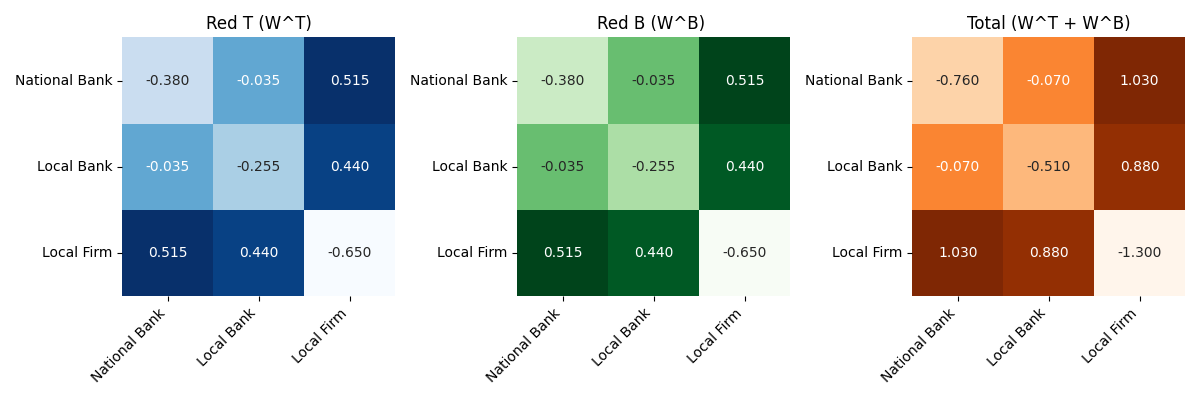
\includegraphics[width=\textwidth,height=1\textheight,keepaspectratio]{sin_rest_titulo.png}
  
  \vspace{0.5em}
  
  % Contenido inferior en dos columnas
  \begin{columns}[T]
    \begin{column}{0.55\textwidth}
      \textbf{Ejemplo Original con el Modelo Extendido}
      \begin{itemize}
        \item Sin restricciones
        \item Sin beneficio por transparencia  
        \item Sin fricción en red blockchain
      \end{itemize}
    \end{column}
    \begin{column}{0.55\textwidth}
      \begin{table}[h]
        \centering
        \begin{tabular}{|l|c|}
          \hline
          Volumen (T)     & 3.265 \\
          \hline
          Volumen (B)     & 3.265 \\
          \hline
          Volumen Total   & 6.530  \\
          \hline
          \% adopción B    & 50\% \\
          \hline
        \end{tabular}
      \end{table}
    \end{column}
  \end{columns}
  
\end{frame}


\begin{frame}{Replicación Ejemplo 5 del Modelo Original}
  
  % Imagen principal
  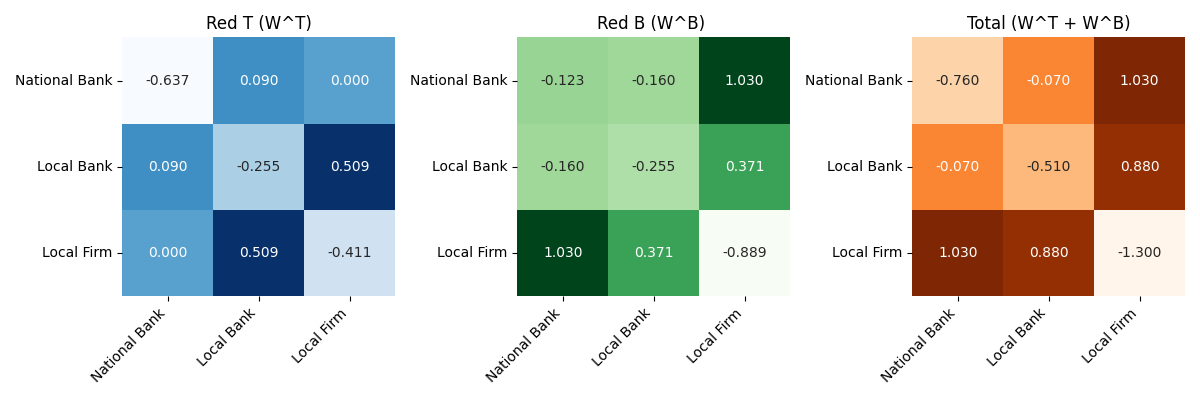
\includegraphics[width=\textwidth,height=1\textheight,keepaspectratio]{con_rest_titulo.png}
  
  \vspace{0.5em}
  
  % Contenido inferior en dos columnas
  \begin{columns}[T]
    \begin{column}{0.55\textwidth}
      \textbf{Ejemplo Original con el Modelo Extendido}
      \begin{itemize}
        \item Con restricciones (Banco Local - Firma Local)
        \item Sin beneficio por transparencia  
        \item Sin fricción en red blockchain
      \end{itemize}
    \end{column}
    \begin{column}{0.55\textwidth}
      \begin{table}[h]
        \centering
        \begin{tabular}{|l|c|}
          \hline
          Volumen (T)     & 2.5004 \\
          \hline
          Volumen (B)     & 4.3884 \\
          \hline
          Volumen Total   & 6.8888  \\
          \hline
          \% adopción B    & 63.7\% \\
          \hline
        \end{tabular}
      \end{table}
    \end{column}
  \end{columns}
  
\end{frame}

\begin{frame}{Efectos de $\lambda$ y $\tau$ en el Ejemplo 5 del Modelo Original}

  \begin{figure}
    \centering
    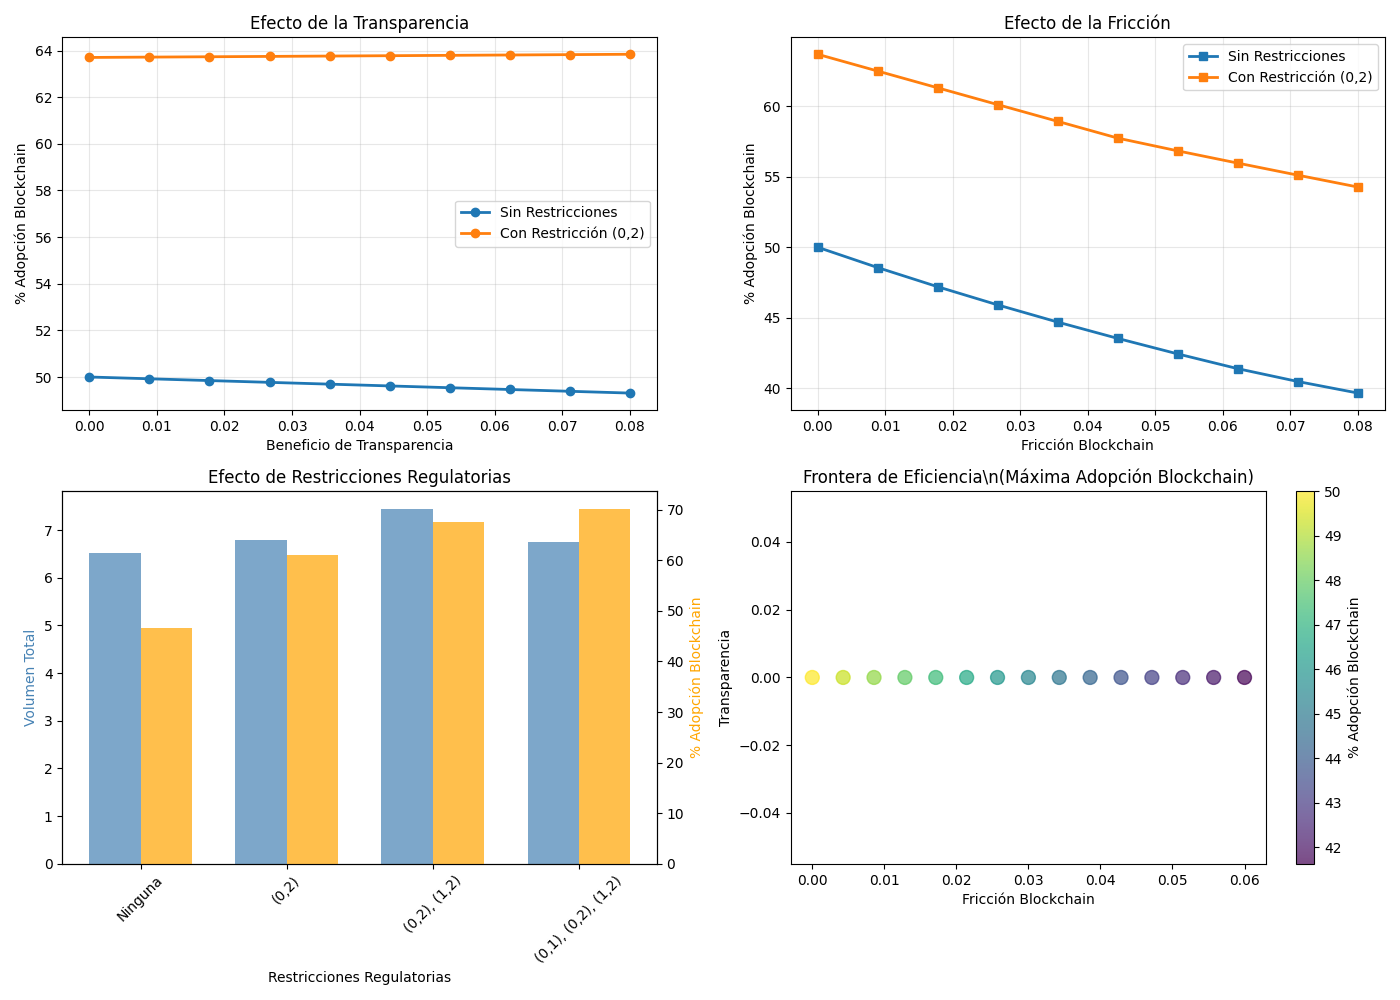
\includegraphics[width=0.95\textwidth]{ex5tauylambda.png}
    
  \end{figure}
\end{frame}


\begin{frame}{Resultados del Modelo Extendido}
Se realizaron 2000 simulaciones con matrices de retorno esperado y covarianzas aleatorias, los resultados fueron los siguientes:
\begin{itemize}
    \item Adopción baseline: 50.00\%
    \item Transparencia ($\tau=0.1$): +1.53 pp
    \item Fricción ($\lambda_B=0.1$): -12.13 pp
    \item Restricciones: +5.35 pp
\end{itemize}
\end{frame}

\begin{frame}{Resultados}
  
  \begin{columns}[T]
    
    % Primera columna - Transparencia
    \begin{column}{0.32\textwidth}
      \centering
      \textcolor{blue}{\textbf{¿TRANSPARENCIA AUMENTA ADOPCIÓN?}}
      
      \vspace{0.5em}
      
      \begin{itemize}
        \item H0: $\tau$ no tiene efecto positivo en adopción
        \item p-value: 0.000001
      \end{itemize}
      
      \vspace{1em}
      
      La transparencia tiene \textbf{efecto positivo} en la adopción de blockchain.
    \end{column}
    
    % Segunda columna - Fricción
    \begin{column}{0.32\textwidth}
      \centering
      \textcolor{blue}{\textbf{¿FRICCIÓN AUMENTA ADOPCIÓN?}}
      
      \vspace{0.5em}
      
      \begin{itemize}
        \item H0: $\lambda$B no reduce adopción
        \item p-value: 0.000000
      \end{itemize}
      
      \vspace{1em}
      
      La fricción tiene \textbf{efecto negativo} en la adopción de blockchain.
    \end{column}
    
    % Tercera columna - Restricciones
    \begin{column}{0.35\textwidth}
      \centering
      \textcolor{blue}{\textbf{¿RESTRICCIONES AUMENTAN ADOPCIÓN?}}
      
      \vspace{0.5em}
      
      \begin{itemize}
        \item H0: Restricciones no aumentan adopción blockchain 
        \item p-value: 0.000029
      \end{itemize}
      
      \vspace{1em}
      
      Las restricciones tienen \textbf{efecto positivo} en la adopción de blockchain.
    \end{column}
    
  \end{columns}
  
\end{frame}

\begin{frame}{Resultados}
  \begin{columns}[T]
    % Primera columna - Efectos de Fricción
    \begin{column}{0.48\textwidth}
      \centering
      \textbf{Efectos de Fricción ($\tau$=0)}
      
      \vspace{0.3em}
      
      \small{Adopción Baseline ($\lambda$B=0, $\tau$=0): 50.00\%}
      
      \vspace{0.5em}
      
      \begin{table}[h]
        \centering
        \begin{tabular}{|c|c|c|}
          \hline
          \textbf{$\lambda_B$} & \textbf{\% adop.} & \textbf{Var.} \\
          \hline
          0.0 & 50.00 & +0.00 pp \\
          \hline
          0.02 & 44.66 & -5.34 pp \\
          \hline
          0.1 & 37.87 & -12.13 pp \\
          \hline
          0.2 & 35.83 & -14.17 pp \\
          \hline
          0.5 & 29.83 & -20.17 pp \\
          \hline
        \end{tabular}
      \end{table}
    \end{column}
    
    % Segunda columna - Efectos de Transparencia
    \begin{column}{0.5\textwidth}
      \centering
      \textbf{Efectos de Transparencia ($\lambda$B=0)}
      
      \vspace{0.3em}
      
      \small{Adopción Baseline ($\lambda$B=0, $\tau$=0): 50.00\%}
      
      \vspace{0.5em}
      
      \begin{table}[h]
        \centering
        \begin{tabular}{|c|c|c|}
          \hline
          \textbf{$\tau$} & \textbf{\% adop.} & \textbf{Var.} \\
          \hline
          0.0 & 50.00 & +0.00 pp \\
          \hline
          0.02 & 51.32 & +1.32 pp \\
          \hline
          0.1 & 51.53 & +1.53 pp \\
          \hline
          0.2 & 51.70 & +1.70 pp \\
          \hline
          0.5 & 53.41 & +3.41 pp \\
          \hline
        \end{tabular}
      \end{table}
    \end{column}
  \end{columns}
\end{frame}

\begin{frame}{Resultados}
  \begin{columns}[T]
    \begin{column}{0.55\textwidth}
      \centering
      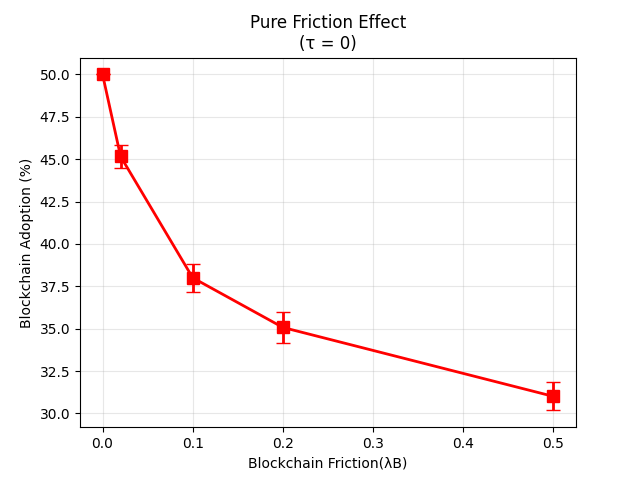
\includegraphics[width=\textwidth]{friction.png}
    \end{column}
    \begin{column}{0.55\textwidth}
      \centering
      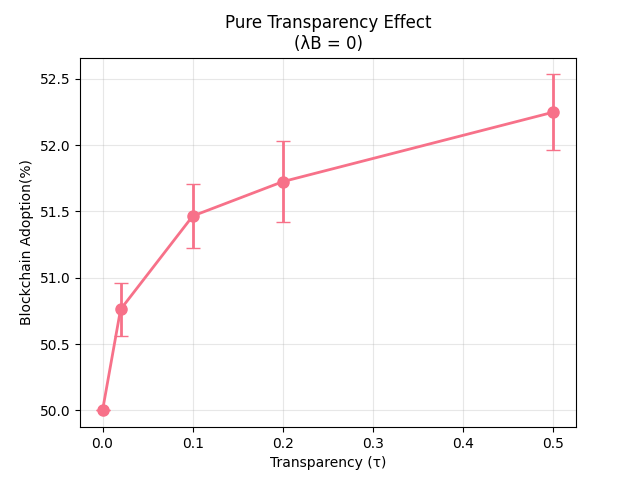
\includegraphics[width=\textwidth]{transp.png}
    \end{column}
  \end{columns}
\end{frame}

\begin{frame}{Trabajo Actual}
\begin{itemize}
\item Revisión algebraica de los resultados numéricos
    \begin{itemize}
        \item Verificación matemática de consistencia entre derivaciones teóricas y simulaciones.
        \item Validación de propiedades de convergencia y teoremas.
    \end{itemize}
\item Calibración de nuevos parámetros.
    \begin{itemize}
        \item Estimación empírica de $\tau$.
        \item Calibración de $\lambda$.
    \end{itemize}
\item Ajuste del modelo a datos de donaciones.
\end{itemize}
\end{frame}


\end{document}